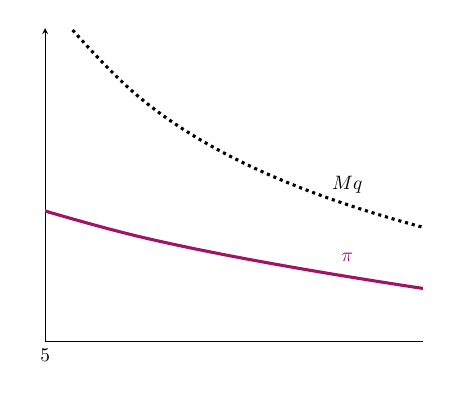
\begin{tikzpicture}[scale=0.7]
\begin{axis}[
                xlabel=\empty,
                x axis line style={opacity=100},
                ylabel=\empty,
                xmin=5, xmax=10,
                ymin=0, ymax=1,
                axis y line=left,
                y axis line style={opacity=100},
                ytick={1.4487},
                xtick={5},
                xticklabels={5},
                yticklabels={$\phi(5)$},
                axis x line*=bottom
                        ]
 \addplot[domain=0:150, RedViolet, ultra thick,smooth] {e^(-x*0.1)-0.2};
 \addplot[domain=0:150, black, ultra thick,smooth,dotted] {e^(-x*0.2+1)};
 \node[align=left] at (9,0.5) {$Mq$};
 \node[align=left, RedViolet] at (9,0.27) {$\pi$};
\end{axis}
\end{tikzpicture}